\documentclass[12pt, handout]{beamer}

\usetheme{Boulder}


\title{Unit testing with IDL}
\subtitle{Using mgunit to unit test code in IDL}
\author{Michael D. Galloy}
\institute[Tech-X Corporation]{Tech-X Corporation\\ Boulder, CO}
\titlegraphic{
\includegraphics[width=1.5cm]{TechX_logo.png}\hspace*{7.5cm}~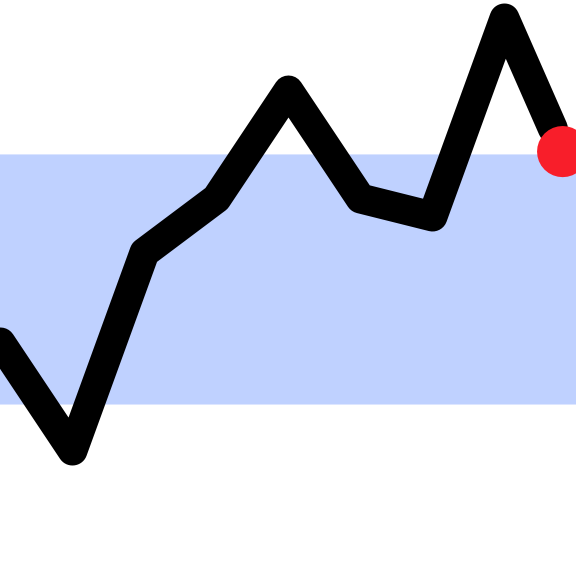
\includegraphics[width=1.5cm]{favicon-nogrid.png}}
%\logo{
\includegraphics[width=1cm]{TechX_logo.png}}

\date{11 November 2013}


\begin{document}


\begin{frame}[plain]
  \titlepage
\end{frame}


\section{Introduction}
\subsection*{}

\begin{frame}
  \tableofcontents
\end{frame}

\begin{frame}[t, fragile]
  \frametitle{mgunit project}
  \begin{itemize}
    \item Available on GitHub:

\begin{lstlisting}
  github.com/mgalloy/mgunit
\end{lstlisting}

    \item how old?
    \item Goal: quick and easy, name conventions over explicit specifications
  \end{itemize}
\end{frame}


\section{Using mgunit}
\subsection{Basics}

\begin{frame}[t]{Basics}
  \begin{enumerate}
    \item tests and test cases
    \item assert (msg with format codes)
    \item skipping
  \end{enumerate}
\end{frame}

\begin{frame}[t]{Advanced}
  \begin{enumerate}
    \item test suites
    \item fixtures (memory leaks)
    \item test runners
  \end{enumerate}
\end{frame}


\section{Examples}
\subsection*{}

\begin{frame}[t, fragile]
  \hypertarget{examples}{}
  \frametitle{Examples}
  Examples will come from:

  \begin{description}
    \item[GPULib] CUDA bindings for IDL
\begin{lstlisting}
  txcorp.com/home/gpulib
\end{lstlisting}
\hyperlink{gpulib}{\beamergotobutton{go to GPULib}}

    \item[mglib] My personal library for analysis, file I/O, visualization, collections, utility routines, string manipulation, \ldots
\begin{lstlisting}
  gitgub.com/mgalloy/mglib
\end{lstlisting}
  \end{description}
\end{frame}

\begin{frame}[t, fragile]
  \frametitle{Example slide}
\end{frame}


\section{Conclusion}

\subsection{Tips}
\begin{frame}[t]{Tips}
  \begin{enumerate}
    \item use something (hopefully mgunit) {\em regularly}
    \item follow the name conventions
    \item inherit from a subclass of MGutTestCase
    \item skipping is useful
  \end{enumerate}
\end{frame}

\subsection{Future work}
\begin{frame}[t]{Future work}
  \begin{enumerate}
    \item mgunit is fairly mature and not many extra features are currently planned
    \item may be integrated into docs in some way, but that will probably be a feature of IDLdoc and separate from mgunit
  \end{enumerate}
\end{frame}

\begin{frame}{Thanks!}
  \begin{center}

{\huge Questions?} \\

\bigskip

{mgalloy@txcorp.com} \\
{michaelgalloy.com} \\
{@mgalloy}

\end{center}
\end{frame}

% for extra slides
\appendix

\begin{frame}{GPULib}
\hypertarget{gpulib}{}

\hyperlink{examples}{\beamergotobutton{go to Examples}}
\end{frame}

\end{document}
